\chapter{Background}
\label{background}

\section{Introduction to Machine Learning}
In \textcite{MLANN}, Machine Learning is defined as "the question of how to
construct computer programs that automatically improve with experience".
Machine Learning has blossomed in recent years with applications across multiple
domains using vastly different paradigms and technologies.

There are many ways in which Machine Learning can be used in the modern world,
many of which are being utilised to great affect.
Some of these applications, are image recognition, natural language processing,
medical diagnosis and many more.
There may be fear that Machine Learning will start to take away many jobs from
humans but this may not be the case. Imagine a doctor, having to diagnose a
patient, a machine can offer suggestions based on very large datasets of what
the diagnosis is. This is not to say that a Machine would be
perscribing patients, but merely act as an assistant to the doctor.

Machine Ethics is a large problem that comes hand in hand with Machine Learning.
There is a very important question of who takes the blame when things go wrong,
that is why I think it is important that we only use Machine Learning to advise
and not to determine but this can be very difficult in a world where, for
example, an autonomous car has to decide between crashing into a vehicle beside
them with an unknown number of people inside or the two children playing in the
street.

One of the most exciting avenues in Machine Learning, in my opinion, is Computer
Vision. Computer Vision can be used in many areas to improve our lives. As
mentioned earlier, autonomous cars are only possible when a machine can
determine what objects are around it. Computer Vision can allow a machine to
recognise skin diseases in an image. The applications are nearly limitless and
that is without taking into account other uses.

\section{Machine Learning Paradigms}
There are many Machine Learning paradigms, all of which I will
discuss briefly below, but the main area of my focus for this project is in
Artificial Neural Networks (ANN). This is because I have researched extensively into Convolutional Neural Networks which are based on ANN's.
\subsection{Artificial Neural Networks}
An Artificial Neural Network is a bio-inspired system that is used to model the human brain in how it learns from experience.
The ANN uses this model to build a very complex web of connected units called
artificial neurons.
These nuerons are connected by certain weights which determines the processing
capacity of the network and these weights are created by learning a
dataset.(Malachy)
An ANN has a set of inputs that take in a value, sometimes from network outputs
and produce a single result or classification.
While an ANN is bio-inspired from the human brain, there are many elements of
the brain that are not present in ANN and many new elements in ANN that are not
modelled from the human brain.

Before I can talk about Convolution Neural Networks which are vital the image
processing, I will have to talk about the perceptron learning algorithm, the multi
layer percepton, and backpropogation.

\subsubsection{Perceptron Learning - Artificial Neuron}
In our Artificial Neural Network a Perecptron is an Artificial Neuron.
It is called an Artifical Neuron because it is a bio-inspired neuron which models
a neuron in the human brain in terms of inputs and output.

In Perceptron learning, we can take two inputs which are put towards an
activation function with a bias attached as seen in \ref{fig:perceptron}.
These inputs are multiplied by the weights that connect the input to the
activation function and depending on the result, the activation function may
fire an output.

\begin{figure}
     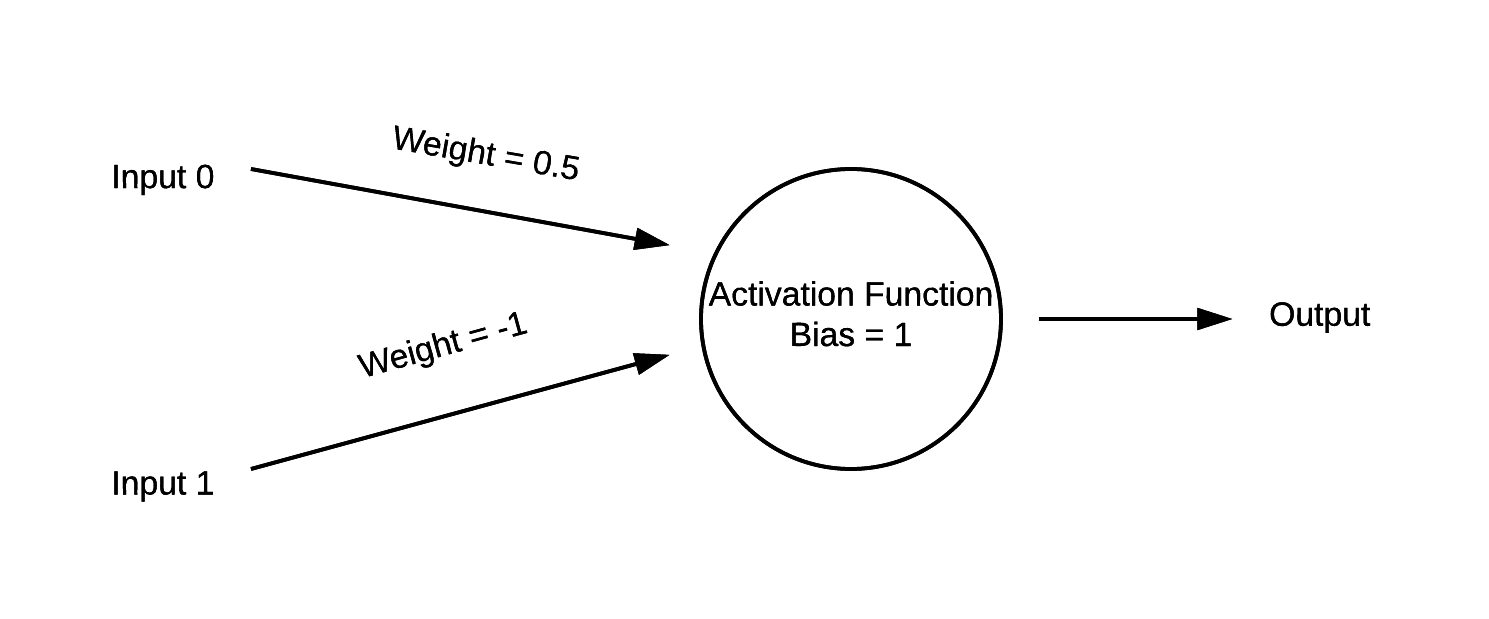
\includegraphics{Perceptron}
     \caption{Perceptron}
     \label{fig:perceptron}
\end{figure}

This Perceptron Learning Rule assumes that there are two sets of instances, a
positive and negative set, and each of these has an input and output domain.

\subsubsection{Multi Layered Perceptron}
Multi Layer Perceptrons (MLP) are made up of multiple layers of perceprons connected
together.
Firstly, we have an input layer, followed by one of more hidden layers and then
finally an output layer.
Any Neural Network with more than three hidden layers is categorised as a deep
layer.

Multi Layer Perceptrons are a class of feed forward Artificial Neural Networks.
These means that the output of each perceptron feeds into an input in the next
layer of the network.

\begin{figure}
    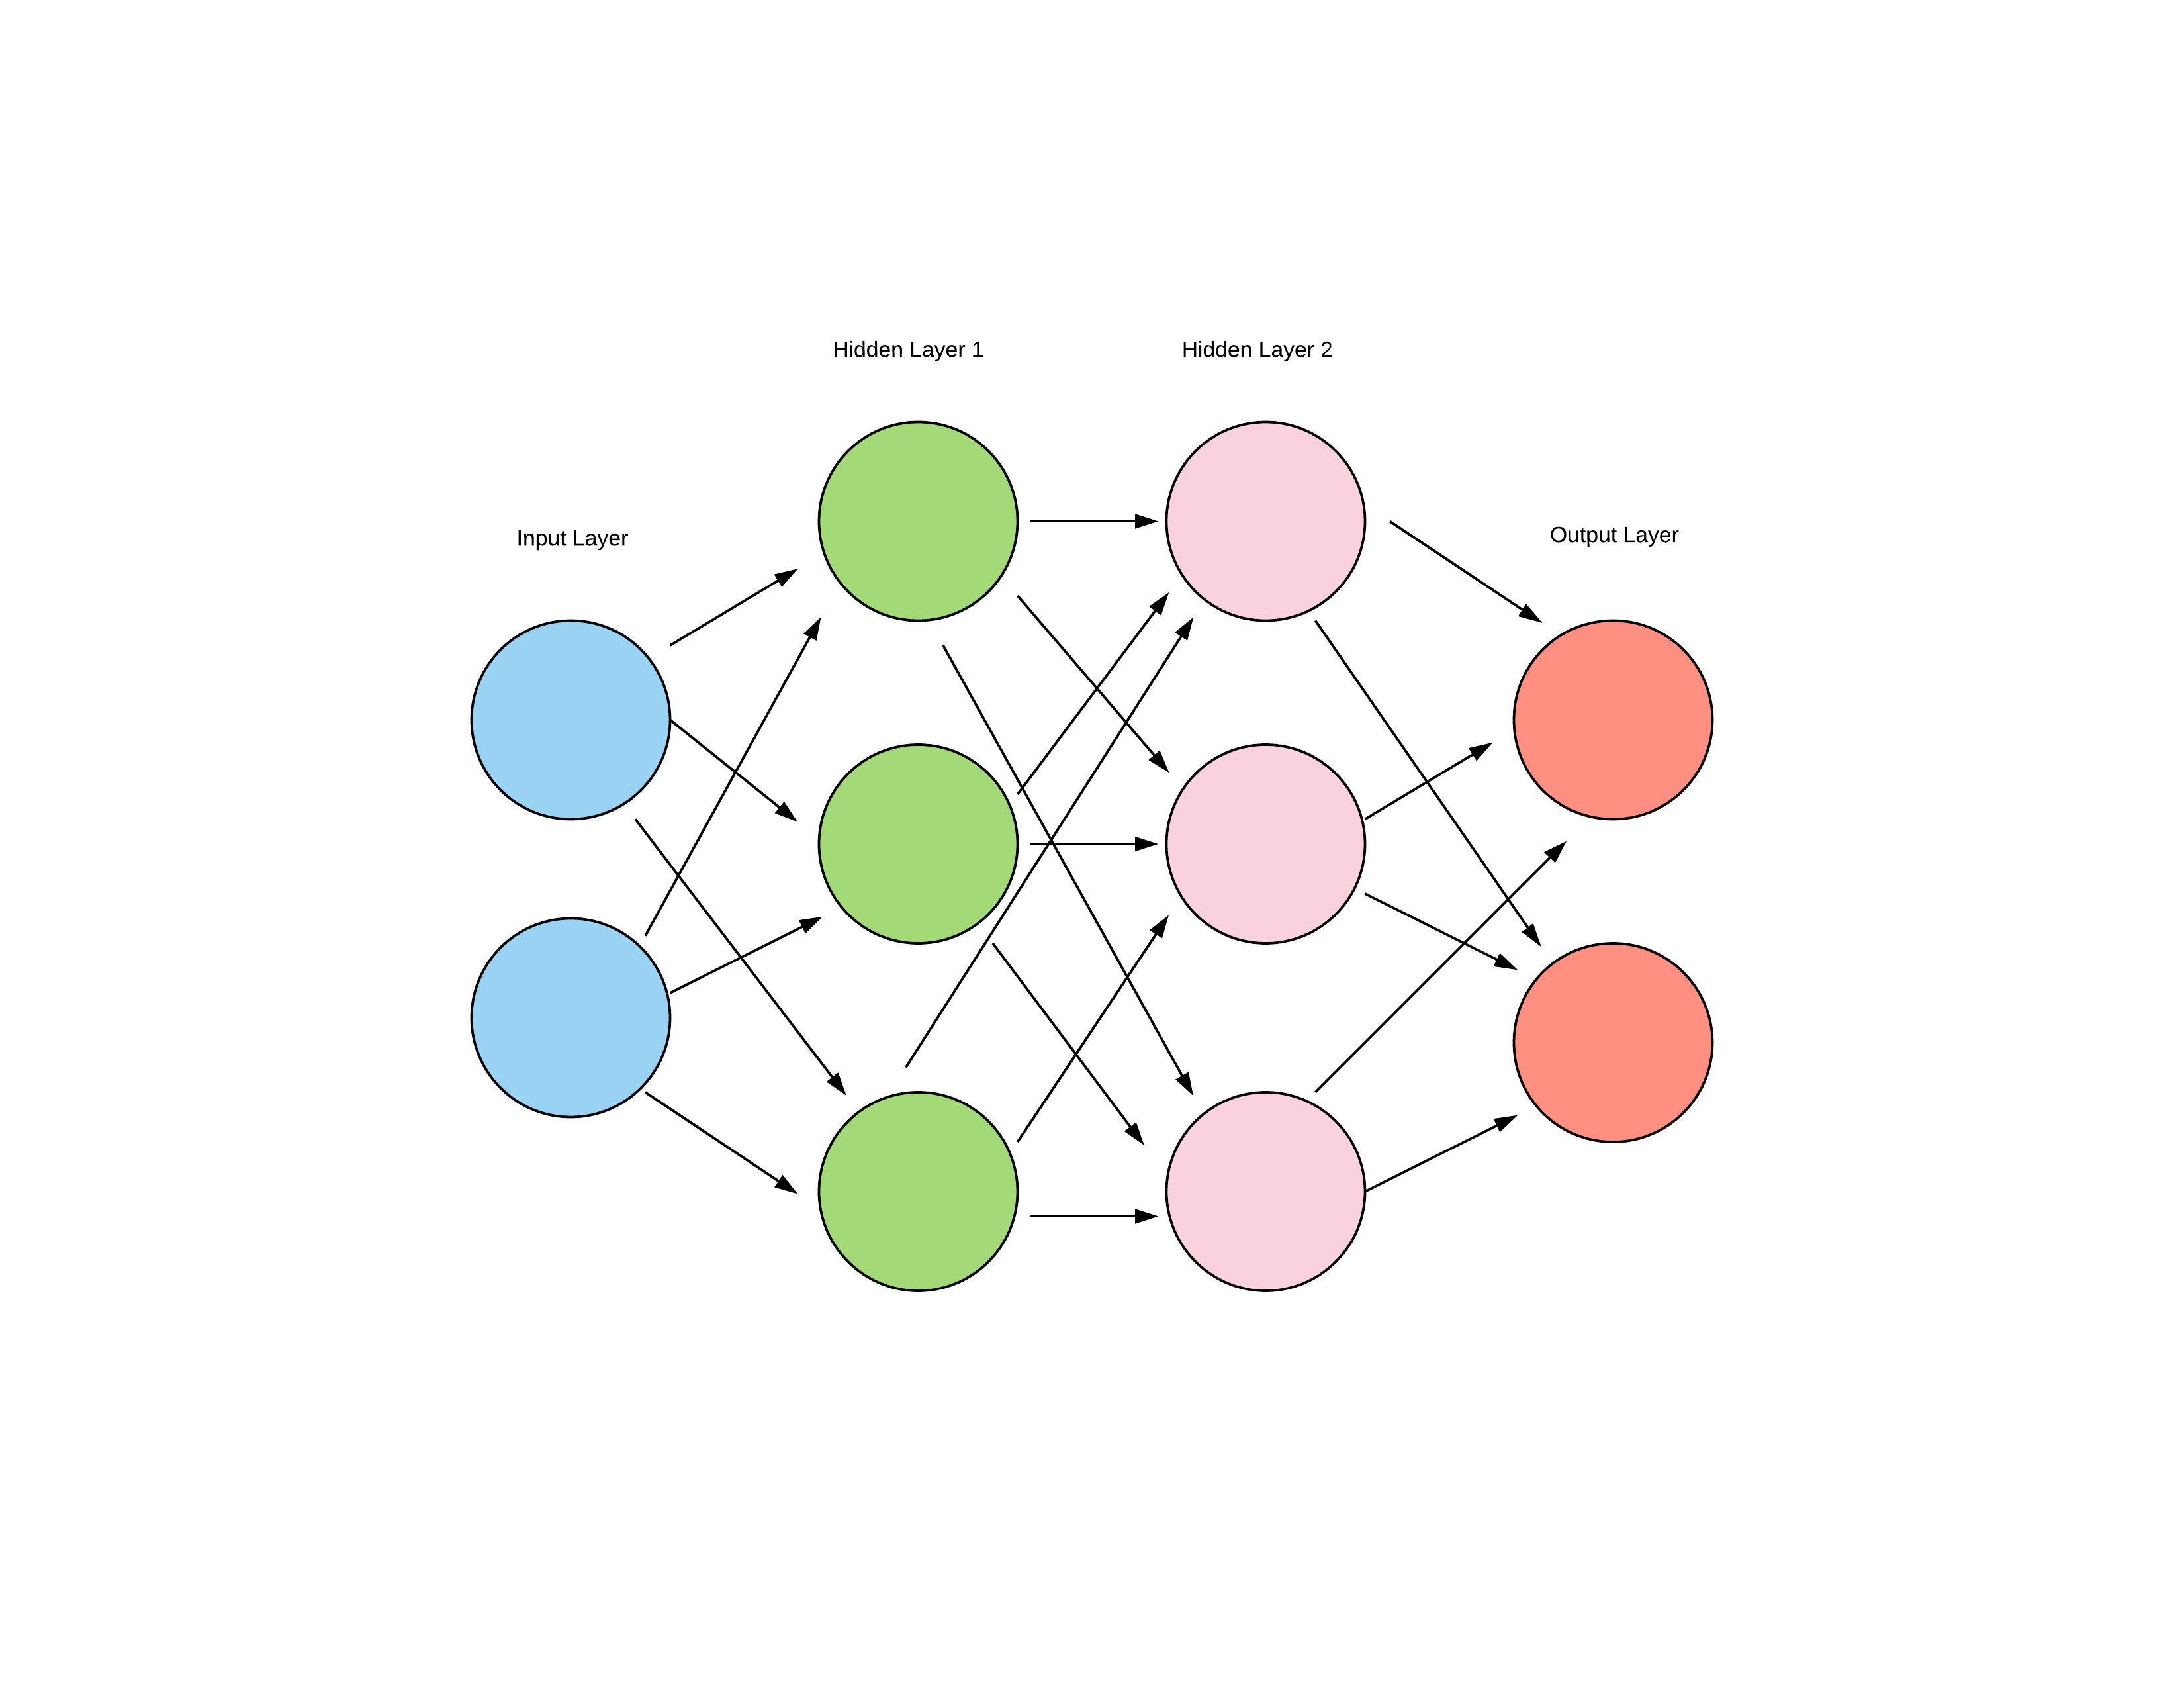
\includegraphics[width=150mm,scale=0.5]{mlp}
     \caption{Multi Layer Perceptron}
     \label{fig:mlp}
\end{figure}

\subsubsection{Gradient Descent and Backpropogation}

\subsubsection{Convolutional Neural Networks}
Convolutional Neural Networks (CNN's) are essentially a Multi Layered Percetron with a
special structure. CNN's have one major difference from a MLP, they have extra
layer of convolution and pooling.

Figure \ref{fig:XtoRec} show an image that we want to compare against
Figure \ref{fig:XtoComp}.
For humans, it is quite easy to determine that these images are very similar but
for a computer this task is surprisingly difficult.

So what a CNN does, to combat this problem, is to take a small feature from
Figure \ref{fig:XtoRec} and compare it to a subsection of Figure \ref{fig:XtoComp}.
The CNN multiplies the feature and a section of Figure \ref{fig:XtoComp}, adds
up the results and divides by 9. This then gives a decimal value of how likely
it is that the feature is in the part of the image, as seen in Figure
\ref{fig:convoluted}.
This is called filtering. The Convolutional layer is composed of carrying out
this filtering for every single possible location in Figure \ref{fig:XtoComp}.
\begin{figure}
      \begin{subfigure}[b]{0.4\textwidth}
          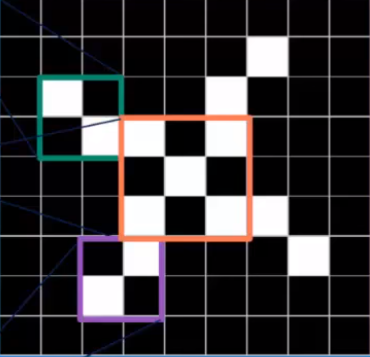
\includegraphics[width=\textwidth]{XtoRec}
          \caption{Image to Classify}
          \label{XtoRec}
      \end{subfigure}
    %
      \begin{subfigure}[b]{0.4\textwidth}
      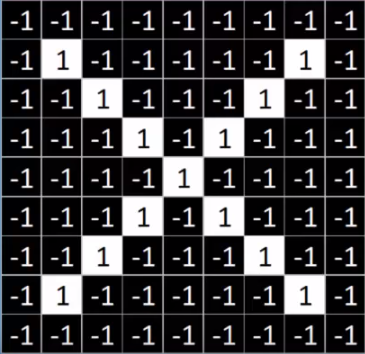
\includegraphics[width=\textwidth]{XtoComp}
      \caption{Image to Compare}
      \label{XtoComp}
      \end{subfigure}
\end{figure}

\begin{figure}
      \begin{subfigure}[b]{0.4\textwidth}
          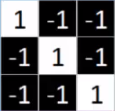
\includegraphics[width=\textwidth]{ImageFeature}
          \caption{Image Feature to Search}
          \label{fig:feature}
      \end{subfigure}
     %
      \begin{subfigure}[b]{0.4\textwidth}
           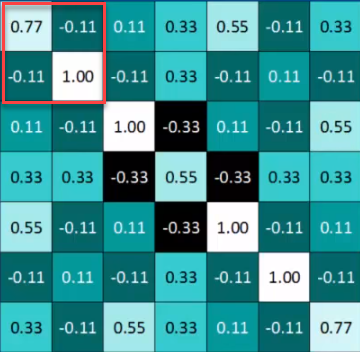
\includegraphics[width=\textwidth]{ConvImage}
           \caption{Convoluted Image}
           \label{fig:convoluted}
      \end{subfigure}
\end{figure}
\begin{figure}
    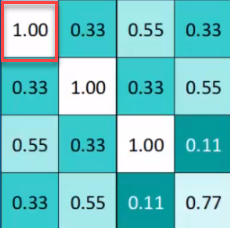
\includegraphics[width=50mm,scale=0.5]{PooledImage}
    \caption{Pooled Image}
    \label{fig:pooled}
\end{figure}
Next is the Pooling Layer, what this layer does, is it takes the convoluted
layer output, you can use Figure \ref{fig:convoluted} as reference, and from a
user defined size ie. 2x2, gets either the highest decimal value (Max pooling)
or the average value (Mean pooling) and records that as the new value for the
section. This is then applied to the entire image. As we can see in Figure
\ref{fig:pooled} we know have a much smaller image stack in which to classify,
thus making the computation easier.

In between the Convolution and Pooling layer, there is sometimes a Normalization
layer. This Normalization layer creates Rectified Linear Units (RLU's). In other
words, if we take Figure \ref{fig:convoluted}, it changes all minus values to
zero.

\subsubsection{Fully Convolutional Networks}
A Fully Convolutional Network is one that does not have a fully connected layer
and in a fully connected layers place is another convolution layer.

\subsection{Other Paradigms}
There are many other Machine Learning paradigms apart from Neural Networks, each of which I will give a brief
introduction.

\subsubsection{Decision Trees}
"Decision tree learning is  method for approcimating disrete-valued target
functions, in which the learned function is represented by a descision tree"
\textcite{MLDT}. There are many different classification algorithms that can
create decision trees from supervised learning.

\subsubsection{Meta/Ensemble Classifiers}
\subsubsection{Logistic Regression}
\subsubsection{Support Vector Machine}
\subsubsection{Regression Analysis}
\subsubsection{Unsupervised Learning}
\subsubsection{Reinforcement Learning}

\section{Overview of Machine Vision Approaches to Identification and Classification}
There have been many attempts of identification and classification by many
different researchers over the last number of years. There some approaches that
decouple the two tasks of identification and classification from one another but
mostly, researchers have attempted the two together. Sometimes, by semantic
segmentation and in others simply building a classifier for the image without
taking into account, the need for object identification.

\subsection{Region Based Convolutional Neural Networks}
Due to the issues with composite images (images with multiple items) in food image recognition, an object detection approach may prove to be successful.
If the objects (different food items) in an image could be classified seperately then the overall effiency of a nutrional assessment system, aided by deep learning, could be improved.
Ross Girshik and other contributors had some very positive results in the area
of object detection using region based convolutional neural networks. There were
four iterations of papers based on this work by Ross and groups in UC Berkley,
Microsoft and Facebook. A PHD student at the time of Ross's first paper also
completed his dissertation on the subject. These papers, their
results (Table \ref{rcnnResults}) and the changes made through each iteration will be analysed thoroughly in the proceeding sections.

In the first paper written by Ross Girshik, while researching at UC Berkeley,
focused on two main insights. These were that " one can apply high-capacity convolutional neural networks (CNNs) to bottom-up region proposals in order to localize and segment objects" and that
"when training data is scarce, supervised pre-training for n auxiliary task,
followed by domain-specific fine-tuning, yields a significant performance boost"
\parencite{rcnn}.

The system that they developed followed these steps:
\begin{itemize}
    \item{Take image as input}
    \item{Extract approximately 2000 region proposals from the image}
    \item{Compute fixed length vectors of features for the regions using a convolutional
        neural network}
    \item{Use a Support Vector Machine (SVM) to classify these regions}
    \item{Bounding box regression for final region proposals}
\end{itemize}

This system utilised selective search to gather these region proposals, but they
mention that a sliding-window detector is also an option. Ross Girshik and his
team used the open source Caffe CNN library for this system. The system is quite
efficient and scalable. It is scalable because of the fixed length vector of
features which will remain constant regardless of inputs and additional outputs.
The team evaluated their results on a few metrics and test sets as seen in Table
\ref{rcnnResults}. Explanation of the datasets used can be seen in Table \ref{datasets}.

Ross Girshik's next iteration of work on region based convolution neural
networks took place in Microsoft Research. This paper was titled "Fast R-CNN" as
its aim was to decrease training and testing time "while also increasing
detection accuracy" \parencite{fastRcnn}.

This paper analyses why RCNN \parencite{rcnn} was slow and therefore how it could be improved.
RCNN was classified to be slow because of three main factors:
\begin{itemize}
	\item{There are multiple stages to training as both a CNN and a SVM need to
		be trained.}
	\item{In training of the SVM, each region proposal must be written to disk
		and is therefore expensive.}
	\item{Object detection takes 47 seconds per image}
\end{itemize}

Due to these problems with RCNN, a new algorithm, titled Fast RCNN was proposed.
The architecture is as follows. An image is taken as input along with a
proposal for regions. The image is pushed through convolutional and pooling
layers (using max pooling). A fixed-length vector of features is then extracted
from each region proposal. These vectors are inputted to fully connected
layers for bounding box location prediction.
At detection time, a pass through of the net is all that is needed so this
runtime is significantly less than RCNN.

Due to the success of RCNN and Fast RCNN, Faster RCNN was introduced to combat
the problem of region proposal computation \parencite{fasterRcnn}.
The architecture for this system comprises of two modules. These consist of a
convolutional neural network for region proposals (RPN) which the feeds into a Fast
RCNN detector. These combine to produce a single neural network for object
detection.

Instead of training these networks separately, the team had to look at how to
share layers between the two networks. There were three options available:
\begin{itemize}
    \item{Alternating training whereby RPN is trained, and then used to train
        Fast RCNN. The Fast RCNN network is then used to initialise RPN and the
		process is iterated \parencite{fasterRcnn}. This paper follows this approach.}
    \item{Approximate joint training.}
    \item{Non- approximate joint training.}
\end{itemize}

\begin{table}[h]
    \centering
    \caption{Results from Region Based CNN Research}
    \label{rcnnResults}
    \begin{tabular}{|p{1.5cm}|l|l|l|l|l|l|}
    \hline
                    & \textbf{VOC07} & \textbf{VOC10} & \textbf{VOC11} & \textbf{VOC12} & \textbf{COCO15} &
                    \textbf{COCO16} \\ \hline
                    RCNN        & 58.5\%  & 53.7\%  & 47.9\%  & N/A     & N/A
                    & N/A      \\ \hline
                    Fast RCNN   & 70.0\%  & 68.8\%  & N/A     & 68.4\%  & N/A
                    & N/A      \\ \hline
                    Faster RCNN & 78.8\%  & N/A     & N/A     & 75.9\%  & 42.7\%
                    & N/A      \\ \hline
                    Mask RCNN   & N/A     & N/A     & N/A     & N/A     & N/A
                    & 63.1\%  \\ \hline
    \end{tabular}
\end{table}

\begin{table}[h]
\centering
\caption{Datasets}
\label{datasets}
\begin{tabular}{|p{1.65cm}|p{10.5cm}|}
\hline
\textbf{Table} & \textbf{Explanation}                                                                                                                                                                                               \\ \hline
VOC07          & The PASCAL VOC dataset is used for the PASCAL (Pattern Analysis, Statistical Modelling and Computational Learning) Visual Object Classes Challenge. \parencite{pascal-voc-2007} was used for the 2007 challenge. \\ \hline
VOC10          & The PASCAL VOC 2010 dataset was used for the 2010 challenge \parencite{pascal-voc-2010}.                                                                                                                         \\ \hline
VOC11          & The PASCAL VOC 2011 dataset was used for the 2011 challenge \parencite{pascal-voc-2011}.                                                                                                                        \\ \hline
VOC12          & The PASCAL VOC 2012 dataset was used for the 2012 challenge \parencite{pascal-voc-2012}.                                                                                                                        \\ \hline
COCO15         & The COCO (Common Objects in Context) dataset created by Microsoft (\parencite{coco}) is used to measure the efficacy of object detection algorithms. The COCO 2015 dataset was released in 2015 for training.    \\ \hline
COCO16         & An updated version of the COCO dataset was released in 2015.                                                                                                                                                       \\ \hline
\end{tabular}
\end{table}

The most recent paper on this topic was also written by Ross Girshik while
working with Facebook AI Research \parencite{maskRcnn}. Mask RCNN " extends Faster
RCNN by adding a branch for predicting an object mask in parallel with the
existing branch for bounding box regression" \parencite{maskRcnn}.
Mask RCNN has two modules, like Faster RCNN, where the first module is the
Region Proposal Network. In the second module, in parallel to classification, a
binary mask is outputted for each region. Bounding box regression and
classification are done in parallel.


\subsection{Fully Convolutional Neural Networks for Semantic Segmentation}
\subsection{Image Segmentation}
\subsubsection{Graph Based Segmentation}
\subsubsection{Sift/Surf}
\subsection{Convolutional Neural Networks for Classification}

\subsection{Classification}

\section{Technologies}
\subsection{Tensorflow}
\subsection{Jupyter}

\section{Evaluating the Output}


